\documentclass[10pt]{article}
\usepackage[polish]{babel}
\usepackage[utf8]{inputenc}
\usepackage[T1]{fontenc}
\usepackage{amsmath}
\usepackage{amsfonts}
\usepackage{amssymb}
\usepackage[version=4]{mhchem}
\usepackage{stmaryrd}
\usepackage{graphicx}
\usepackage[export]{adjustbox}
\graphicspath{ {./images/} }

\title{Instrukcja dla zdającego }

\author{}
\date{}


\begin{document}
\maketitle
\(\qquad\)

\begin{center}
\begin{tabular}{|l|l}
\hline
 & MATEAATYKA-poziom podstawowy \\
LSCDN & 10 marca 2020 r \\
\hline
\end{tabular}
\end{center}

\begin{enumerate}
  \item Sprawdź, czy arkusz zawiera 16 stron (zadania 1-34). Ewentualne braki zgłoś przewodniczącemu zespołu nadzorującego egzamin.
  \item Rozwiązania zadań i odpowiedzi zamieść w miejscu na to przeznaczonym.
  \item Odpowiedzi do zadań zamkniętych (1-25) przenieś na kartę odpowiedzi, zaznaczając je w części karty przeznaczonej dla zdającego. Zamaluj pola do tego przeznaczone. Błędne zaznaczenie otocz kółkiem i zaznacz właściwe.
  \item Pamiętaj, że pominięcie argumentacji lub istotnych obliczeń w rozwiązaniu zadania otwartego (26-34) może spowodować, że za to rozwiązanie nie otrzymasz pełnej liczby punktów.
  \item Pisz czytelnie i używaj tylko długopisu lub pióra z czarnym tuszem lub atramentem.
  \item Nie używaj korektora, a błędne zapisy wyraźnie przekreśl.
  \item Pamiętaj, że zapisy w brudnopisie nie będą oceniane.
  \item Możesz korzystać z zestawu wzorów matematycznych, cyrkla i linijki oraz kalkulatora prostego.
  \item Na tej stronie oraz na karcie odpowiedzi wpisz swój kod lub nazwisko i imię - zgodnie z ustaleniami szkolnymi.
  \item Nie wpisuj żadnych znaków w części przeznaczonej dla egzaminatora.
\end{enumerate}

Życzymy powodzenia!

Czas pracy:\\
170 minut

Liczba punktów\\
do uzyskania: \(\mathbf{5 0}\)

\section*{Zadanie 1. (lp)}
Wartość wyrażenia \(x^{2}-y^{2}\) dla \(x=2-\sqrt{2}\) i \(y=2+\sqrt{2}\) jest równa\\
A. \(4 \sqrt{2}\)\\
B. \(-4 \sqrt{2}\)\\
C. \(-8 \sqrt{2}\)\\
D. \(8 \sqrt{2}\)

Zadanie 2. (lp)\\
Dana jest liczba \(a=100^{100}\). Liczba \(b\) stanowi \(1 \%\) liczby \(a\). Wówczas\\
A. \(b=100^{96}\)\\
B. \(b=100^{97}\)\\
C. \(b=100^{98}\)\\
D. \(b=100^{99}\)

Zadanie 3. (lp)\\
Jeżeli \(\log _{2} 18=c\), to \(\log _{2} 3\) jest równy\\
A. \(\frac{c+1}{2}\)\\
B. \(\frac{c-1}{2}\)\\
C. \(\frac{c}{6}\)\\
D. \(-\frac{c}{6}\)

Zadanie 4. (lp)\\
Suma kwadratów dwóch wyrażeń \((1-x) i(x+2)\) jest równa\\
A. \(x^{2}-2 x+5\)\\
B. \(x^{2}+2 x+5\)\\
C. \(x^{2}-2 x+4\)\\
D. \(2 x^{2}+2 x+5\)

Zadanie 5. (lp)\\
Dziedziną funkcji \(f(x)=\frac{1}{(x-2)(3+x)}\) jest zbiór\\
A. \(x \in R \backslash\{2\}\)\\
B. \(x \in R \backslash\{-3,2\}\)\\
C. \(x \in R \backslash\{-3\}\)\\
D. \(x \in R \backslash\{-2\}\)

Zadanie 6. (lp)\\
Liczba (-3) jest rozwiązaniem równania\\
A. \(x^{2}+9=0\)\\
B. \(\frac{x+3}{2}=1\)\\
C. \(\frac{2}{x+3}=0\)\\
D. \(x^{2}-9=0\)

Zadanie 7. (lp)\\
Zbiorem rozwiązań nierówności \(\frac{x-2}{3}-x<2\) jest przedział\\
A. \((-\infty,-4)\)\\
B. \((-4,+\infty)\)\\
C. \((-\infty, 4)\)\\
D. \((4,+\infty)\)

Zadanie 8. (lp)\\
Do wykresu funkcji \(f\) danej wzorem \(f(x)=2^{x}-1\) nie należy punkt o współrzędnych\\
A. \((2,-1)\)\\
B. \((2,3)\)\\
C. \((1,1)\)\\
D. \((0,0)\)

Zadanie 9. (lp)\\
Funkcja \(f(x)=-2(x-4)(2+x)\) jest malejąca w przedziale\\
A. \((-2,4)\)\\
B. \((-\infty, 1)\)\\
C. \(\langle-2,4\rangle\)\\
D. \(\langle 1,+\infty)\)

BRUDNOPIS (nie podlega ocenie)

Zadanie 10. (lp)\\
Wykresem funkcji \(f\) danej wzorem \(f(x)=-2(x+2 m)^{2}-5\) jest parabola o wierzchołku w punkcie \(P=(4,-5)\). Wówczas\\
A. \(m=2\)\\
B. \(m=-4\)\\
C. \(m=-2\)\\
D. \(m=4\)

Zadanie 11. (lp)\\
Setny wyraz ciągu \(\left(a_{n}\right)\) jest równy 2020. Wzór ogólny na n-ty wyraz ciągu \(\left(a_{n}\right)\) może mieć postać\\
A. \(a_{n}=2 n-2020\)\\
B. \(a_{n}=\frac{n^{2}}{4}-480\)\\
C. \(a_{n}=n^{2}-480\)\\
D. \(a_{n}=2 n+2020\)

Zadanie 12. (lp)\\
W ciągu arytmetycznym \(\left(a_{n}\right)\), określonym dla \(n \in N^{+}\)spełniony jest warunek \(a_{5}=2\left(a_{3}-a_{1}\right)+1\). Pierwszy wyraz tego ciągu jest równy\\
A. -1\\
B. 1\\
C. 2\\
D. 3

Zadanie 13. (lp)\\
Dany jest trzywyrazowy ciąg geometryczny o wyrazach dodatnich:(2, \(x \sqrt{2}, 6)\) Wówczas\\
A. \(x=2\)\\
B. \(x=6\)\\
C. \(x=\sqrt{6}\)\\
D. \(x=3 \sqrt{2}\)

Zadanie 14. (lp)\\
Wiadomo, że \(\sin \alpha=\frac{3 \sqrt{5}}{7} i \alpha \in\left(90^{\circ}, 180^{\circ}\right)\). Wynika stąd, że\\
A. \(\cos \alpha=\frac{4}{7}\)\\
B. \(\cos \alpha=-\frac{2}{7}\)\\
C. \(\cos \alpha=\frac{2}{7}\)\\
D. \(\cos \alpha=-\frac{4}{7}\)

Zadanie 15. (lp)\\
Na okręgu o środku w punkcie \(O\) leżą punkty \(A, B, C\) (zobacz rysunek). Odcinek \(A C\) jest średnicą okręgu. Kąt \(A O B\) ma miarę \(64^{\circ}\).

Kąt \(O B C\) ma miarę równą\\
A. \(42^{\circ}\)\\
B. . \(34^{\circ}\)\\
C. \(32^{\circ}\)\\
D. \(44^{\circ}\)\\
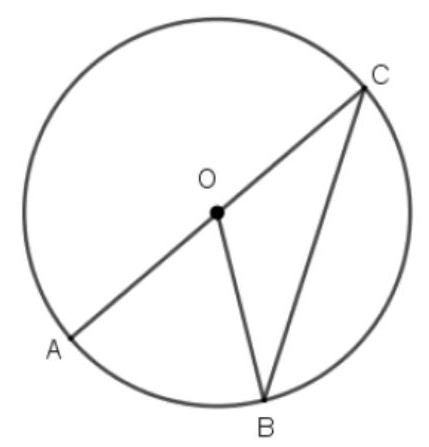
\includegraphics[max width=\textwidth, center]{2024_11_21_c2f4637e26cc7e4291d3g-04(1)}

Zadanie 16. (lp)\\
Dwusieczne kątów ostrych trójkąta prostokątnego \(A B C\) przecinają się w punkcie \(P\). Przyprostokątne \(A B\) i \(B C\) mają długości równe odpowiednio 12 i 9 (zobacz rysunek).

Odległość punktu \(P\) od przeciwprostokątnej \(A C\) jest równa\\
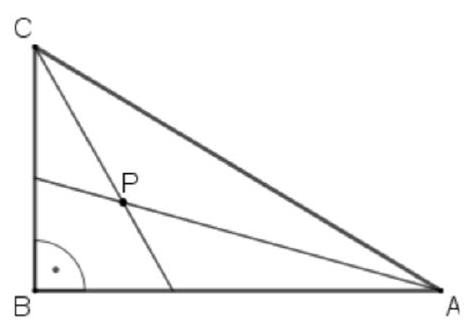
\includegraphics[max width=\textwidth, center]{2024_11_21_c2f4637e26cc7e4291d3g-04}\\
A. 3\\
B. 2\\
C. 15\\
D. \(\frac{15}{2}\)

BRUDNOPIS (nie podlega ocenie)

\section*{Zadanie 17. (lp)}
Obwód trójkąata równobocznego jest równy \(\frac{6 x}{y}\), gdzie \(x>0\) i \(y>0\). Pole powierzchni tego trójkąta jest równe\\
A. \(\frac{x^{2} \sqrt{3}}{y^{2}}\)\\
B. \(\frac{x^{2}}{y^{2}}\)\\
C. \(\frac{3 x}{y}\)\\
D. \(\frac{x \sqrt{3}}{y}\)

Zadanie 18. (lp)\\
Prosta \(k\) o równaniu \(x-y+12=0\), tworzy z osią \(O x\) kąt o mierze równej\\
A. \(30^{\circ}\)\\
B. \(90^{\circ}\)\\
C. \(60^{\circ}\)\\
D. \(45^{\circ}\)

Zadanie 19. (1p)\\
Dłuższy z boków prostokąta \(A B C D\) ma długość równą 12, a dwa sąsiednie wierzchołki mają współrzędne \(C=(-5,1), D=(3,1)\). Pole powierzchni tego prostokąta jest równe\\
A. \(20 \sqrt{3}\)\\
B. 64\\
C. 80\\
D. 96

Zadanie 20. (lp)\\
Przekątna graniastosłupa prawidłowego czworokątnego ma długość równą 16 i jest nachylona do płaszczyzny podstawy pod kątem \(45^{\circ}\). Wysokość tego graniastosłupa ma długość równą.\\
A. 8\\
B. \(8 \sqrt{2}\)\\
C. \(\frac{16 \sqrt{3}}{3}\)\\
D. \(8 \sqrt{3}\)

Zadanie 21. (lp)\\
Wysokość ściany bocznej opuszczona na krawędź podstawy ostrosłupa prawidłowego trójkątnego jest 3 razy dłuższa od krawędzi jego podstawy. Stosunek pola powierzchni bocznej do pola powierzchni podstawy tego ostrosłupa jest równy\\
A. \(\frac{1}{3}\)\\
B. \(2 \sqrt{3}\)\\
C. \(6 \sqrt{3}\)\\
D. 9

Zadanie 22. (lp)\\
Ze zbioru cyfr \(\{6,7,8,9\}\) losujemy kolejno bez zwracania dwie cyfry i tworzymy liczbę dwucyfrową. Prawdopodobieństwo tego, że utworzona liczba będzie nie mniejsza niż 89 jest równe\\
A. \(\frac{3}{16}\)\\
B. \(\frac{4}{16}\)\\
C. \(\frac{3}{12}\)\\
D. \(\frac{4}{12}\)

Zadanie 23. (lp)\\
Średnia arytmetyczna zestawu danych: \(2, x, 4, x, 6, x, 8, x, 10, x\) jest równa 4,5. Mediana tego zestawu danych wynosi\\
A. 2\\
B. 2,5\\
C. 3\\
D. 3,5

Zadanie 24. (lp)\\
Pole powierzchni całkowitej sześcianu jest równe 72. Wynika stąd, że przekątna tego sześcianu ma długość równą\\
A. 6\\
B. \(2 \sqrt{3}\)\\
C. \(3 \sqrt{3}\)\\
D. 12

BRUDNOPIS (nie podlega ocenie)

\section*{Zadanie 25. (lp)}
Aby odblokować telefon komórkowy należy użyć czterocyfrowego kodu PIN. Paweł ustalił, że jego kod PIN na parzystych miejscach będzie miał cyfrę nieparzystą, a na nieparzystych miejscach cyfrę parzystą oraz cyfry nie będą się powtarzać. Ile różnych kodów PIN może utworzyć Paweł?\\
A. 400\\
B. 300\\
C. \(2 \cdot 5^{4}\)\\
D. \(2 \cdot 4^{5}\)

BRUDNOPIS (nie podlega ocenie)

\section*{LUBELSKA PRÓBA PRZED MATURĄ 2020 - poziom podstawowy}
\section*{ZADANIA OTWARTE}
Rozwiązania zadań o numerach od 26 do 34 należy zapisać \(w\) wyznaczonych miejscach pod treścia zadania (pamiętaj o udzieleniu odpowiedzi)

Zadanie 26. (2p)\\
Rozwiąż nierówność \(2 x^{2}-7 x \geq-5\).\\

\includegraphics[max width=\textwidth, center]{2024_11_21_c2f4637e26cc7e4291d3g-09(1)}

Zadanie 27. (2p)\\
Uzasadnij, że jeśli \(a \neq 0\) oraz \(\frac{b^{2}}{a^{2}}=2 b-a^{2}\), to \(b=a^{2}\)

\section*{Zadanie 28. (2p)}
Dany jest prostokąt \(A B C D\), w którym jeden bok jest dwa razy dłuższy od drugiego. Na boku DC zbudowano trójkąt równoboczny CDE (patrz rysunek). Punkt \(K\) jest takim punktem odcinka CE, że kąt \(B K C=75^{\circ}\). Udowodnij, że punkt \(K\) jest środkiem odcinka \(C E\).\\
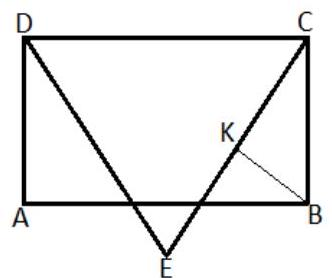
\includegraphics[max width=\textwidth, center]{2024_11_21_c2f4637e26cc7e4291d3g-09}

\section*{LUBELSKA PRÓBA PRZED MATURĄ 2020 - poziom podstawowy}
Zadanie 29. (2p)\\
Ile jest liczb naturalnych dwucyfrowych podzielnych przez 15 lub 20?\\

\includegraphics[max width=\textwidth, center]{2024_11_21_c2f4637e26cc7e4291d3g-10(1)}

Zadanie 30. (2p)\\
Pierwszy wyraz ciągu arytmetycznego jest równy 3 , a czwarty jest równy 15 . Oblicz sumę sześciu początkowych wyrazów tego ciągu.\\

\includegraphics[max width=\textwidth, center]{2024_11_21_c2f4637e26cc7e4291d3g-10}

Zadanie 31. (2p)\\
Punkty \(A=(-3,-5), B=(4,-1), C=(-2,3)\) są wierzchołkami trójkąta równoramiennego. Oblicz długość ramienia tego trójkąta.

\section*{LUBELSKA PRÓBA PRZED MATURĄ 2020 - poziom podstawowy}
Zadanie 32. (4p)\\
Wierzchołki trójkąta \(A B C\) leżą na paraboli, która jest wykresem pewnej funkcji kwadratowej \(f\) (zobacz rysunek).\\
Pole tego trójkąta jest równe 8 , punkt \(C=(1,4)\) jest wierzchołkiem paraboli, a punkty \(A\) i \(B\) leżą na osi \(O x\). Wyznacz wzór funkcji \(f\).\\
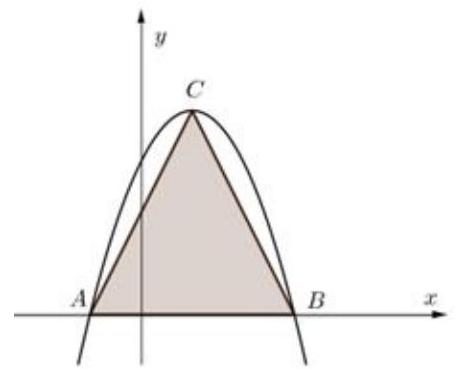
\includegraphics[max width=\textwidth, center]{2024_11_21_c2f4637e26cc7e4291d3g-11}

\section*{LUBELSKA PRÓBA PRZED MATURĄ 2020 - poziom podstawowy}
Zadanie 33. (4p)\\
Dane są dwa pojemniki. W pierwszym z nich znajduje się 9 kul: 4 białe, 3 czarne i 2 zielone. W drugim pojemniku znajduje się 6 kul: 2 białe, 3 czarne i 1 zielona. \(Z\) każdego pojemnika losujemy po jednej kuli. Oblicz prawdopodobieństwo wylosowania dwóch kul tego samego koloru.

\section*{LUBELSKA PRÓBA PRZED MATURĄ 2020 - poziom podstawowy}
Zadanie 34. (5p)\\
Podstawą ostrosłupa \(A B C S\) jest trójkąt równoboczny \(A B C\) o boku długości 8 . Punkt \(D\) jest środkiem krawędzi \(A B\), odcinek \(D S\) jest wysokością ostrosłupa. Krawędzie \(A S\) i \(B S\) mają długość 7 . Oblicz długość krawędzi \(C S\) tego ostrosłupa.

BRUDNOPIS (nie podlega ocenie)

BRUDNOPIS (nie podlega ocenie)

\section*{KARTA ODPOWIEDZI}
\(\square\) Nazwisko i imię

Wypelnia piszacy

\begin{center}
\begin{tabular}{|c|c|c|c|c|}
\hline
\( \begin{gathered} \mathrm{Nr} \\ \text { zadanias } \end{gathered} \) & A & B & C & D \\
\hline
1. & ㅁ & ㅁ & ㅁ & ㅁ \\
\hline
2. & ㅁ & ㅁ & ㅁ & ㅁ \\
\hline
3. & ㅁ & ㅁ & ㅁ & ㅁ \\
\hline
4. & ㅁ & ■ & ■ & ㅁ \\
\hline
5. & ㅁ & ㅁ & ■ & ㅁ \\
\hline
6. & ㅁ & ㅁ & ㅁ & ㅁ \\
\hline
7. & ㅁ & ■ & ㅁ & ㅁ \\
\hline
8. & ㅁ & ㅁ & ㅁ & ㅁ \\
\hline
9. & ㅁ & ㅁ & ㅁ & ㅁ \\
\hline
10. & ㅁ & ㅁ & ㅁ & ㅁ \\
\hline
11. & ㅁ & ㅁ & ㅁ & ㅁ \\
\hline
12. & ㅁ & ■ & ㅁ & ㅁ \\
\hline
13. & ㅁ & ㅁ & ㅁ & ㅁ \\
\hline
14. & ㅁ & ■ & ㅁ & ㅁ \\
\hline
15. & ㅁ & ■ & ㅁ & ㅁ \\
\hline
16. & ㅁ & ㅁ & ㅁ & ㅁ \\
\hline
17. & ㅁ & ㅁ & ㅁ & ㅁ \\
\hline
18. & ㅁ & ㅁ & ㅁ & ㅁ \\
\hline
19. & ㅁ & ㅁ & ㅁ & ㅁ \\
\hline
20. & ㅁ & ■ & ■ & ㅁ \\
\hline
21. & ㅁ & ■ & ■ & ㅁ \\
\hline
22. & ㅁ & ■ & ■ & ㅁ \\
\hline
23. & ㅁ & ㅁ & ■ & ㅁ \\
\hline
24. & ㅁ & ㅁ & ㅁ & ㅁ \\
\hline
25. & ㅁ & ■ & ■ & ㅁ \\
\hline
\multicolumn{3}{|r|}{Razem} &  &  \\
\hline
\end{tabular}
\end{center}

Wypelnia sprawdzający

\begin{center}
\begin{tabular}{|c|c|c|c|c|}
\hline
\begin{tabular}{c}
Nr \\
zadruia \\
\end{tabular} & X & 0 & 1 & 2 \\
\hline
26. & \(\square\) & \(\square\) & \(\square\) & \(\square\) \\
\hline
27. & \(\square\) & \(\square\) & \(\square\) & \(\square\) \\
\hline
28. & \(\square\) & \(\square\) & \(\square\) & \(\square\) \\
\hline
29. & \(\square\) & \(\square\) & \(\square\) & \(\square\) \\
\hline
30. & \(\square\) & \(\square\) & \(\square\) & \(\square\) \\
\hline
31. & \(\square\) & \(\square\) & \(\square\) & \(\square\) \\
\hline
\end{tabular}
\end{center}

Razem \(\square\)

\begin{center}
\begin{tabular}{|c|c|c|c|c|c|c|c|}
\hline
\begin{tabular}{c}
Ni \\
zadama \\
\end{tabular} & X & 0 & 1 & 2 & 3 & 4 & 5 \\
\hline
32. & \(\square\) & \(\square\) & \(\square\) & \(\square\) & \(\square\) & \(\square\) &  \\
\hline
33. & \(\square\) & \(\square\) & \(\square\) & \(\square\) & \(\square\) & \(\square\) &  \\
\hline
34. & \(\square\) & \(\square\) & \(\square\) & \(\square\) & \(\square\) & \(\square\) & \(\square\) \\
\hline
\end{tabular}
\end{center}

Razem \(\square\)

\begin{center}
\begin{tabular}{|l|l|}
\hline
Suma punktów & Wynik w\% \\
\hline
 &  \\
 &  \\
\hline
\end{tabular}
\end{center}


\end{document}